\section{Simulerings blokker}
\thispagestyle{fancy}

For å skape eit meir realistisk miljø for testinga lagde vi nokre simuleringsblokker.
Desse blokkene etterliknar driftssituasjonar og gjer simuleringa enklare og meir effektiv.
Vi lagde hovudsakleg to slike blokker; ei simulerer fylling av ein tank
og ei for tilbakemelding frå ventilar.

Blokk for tank simulering er enkel og skriven spesifikt for Sande reinseanlegg, som omfattar ein mottakstank
og to reaktorar.
Det er lite truleg at desse simuleringsblokkene vil bli brukt vidare, men dei gav
oss den realismen vi trengte.

Desse blokkene forenkla også sjølve arbeidet med simuleringa.
Før vi utvikla blokka for tilbakemelding på ventilar, 
gav vi manuelt kvar ventil \gls{XGH} eller \gls{XGL} basert på den faktiske stillinga (open/stengd).
Dette fungerer greitt dersom ein testar små områder eller kunn ei ventilblokk, men
når simuleringa omfatta større delar av programmet blir denne jobben tungvindt og tidkrevjande.

På desse blokkene har vi tatt oss meir friheit i namngiving, feilhandtering osv.,
fordi blokkene ikkje skal brukast når programmet er ferdig stilt.


\begin{figure}[htbp]
    \centering
    \begin{subfigure}[b]{0.3\textwidth}
        \centering
        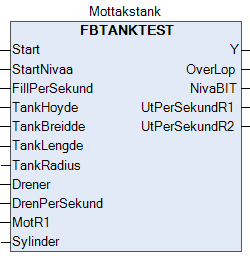
\includegraphics[width=0.9\textwidth]{Figurar/TankSim.png}
        \caption{Tank}\label{fig:TankSim}
    \end{subfigure}
    \hfill
    \begin{subfigure}[b]{0.3\textwidth}
        \centering
        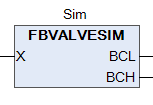
\includegraphics[width=0.9\textwidth]{Figurar/ValveSim.png}
        \caption{Ventil}\label{fig:ValveSim}
    \end{subfigure}
    \caption{Simuleringsblokker}\label{fig:SimuleringsBlokker}
\end{figure}

\newpage